\subsection{Speeded Up Robust Features (SURF)}
Das Folgende Kapitel basiert auf dem Paper ''SURF: Speeded Up Robust Features'' von Herbert Bay.
\footnote{\cite{Bay:2008:SRF:1370312.1370556}}

Das Verfahren ''Speeded Up Robust Features'' (SURF) wurde von Herbert Bay 2006 vorgestellt. SURF ist ein Verfahren, das sowohl Merkmale findet, als auch Deskriptoren für diese bildet.
SURF versucht durch einige Approximationen schneller als SIFT zu sein ohne große Verluste in der Genauigkeit zu haben.

Für schnelle Berechnung von rechteckigen Filtern werden Integralbilder verwendet. Diese ermöglichen eine sehr schnelle Berechnung von Pixelsummen in einem rechteckigen Bildbereich.
In einem Integralbild ist jeder Pixelwert die Summe aller Pixel in einem Rechteck zwischen dem aktuellen Punkt und dem Bildursprung.

\[
I_i(x, y) = \sum_{i = 0}^{i < x} \sum_{j = 0}^{j < y} I(i, j)
\]

Nun kann die Summe der Pixelwerte eines Recktecks
 $R = \{ (x_1, y_1), (x_2, y_2), (x_3, y_3), (x_4, y_4)  \}$ mit nur vier Bildzugriffen berechnet werden.
\[
S(R) = I_i(x_1, y_1) + I_i(x_4, y_4) - I_i(x_2, y_2) - I_i(x_3, y_3)
\]



\subsubsection{Merkmalserkennung}

SURF nutzt die Determinante der Hesse-Matrix um Keypoints zu finden. Die Hesse-Matrix ist die zweite Ableitung einer mehrdimensionalen Funktion. Sie kann somit als ein Maß der Krümmung verstanden werden.
Es wird, ähnlich zu SIFT, in verschiedenen Skalierungen nach Maxima von $det(\mathcal{H}(x, y, \sigma))$ gesucht. Dabei ist die Hesse Matrix $\mathcal{H}(x, y, \sigma)$ für das Bild $I(x, y)$ und die Skalierung $\sigma$ definiert als:

\[
\mathcal{H}(x, y, \sigma) = 
\begin{bmatrix}
L_{xx}(x, \sigma) & L_{xy}(x, \sigma) \\
L_{xy}(x, \sigma) & L_{yy}(x, \sigma)
\end{bmatrix}
\]

Wobei $L_{xx}(x, y, \sigma)$ die Faltung von der zweifachen nach x abgeleiteten Gaußfunktion mit dem Bildpunkt ist. Das gleiche gilt für $L_{xy}(x, y, \sigma)$ und $L_{yy}(x, y, \sigma)$ in die entsprechenden Richtungen.

Um die Determinante schnell berechnen zu können, werden die partiellen Gaußableitungen mit rechteckigen Filtern approximiert. Diese seien im Folgenden $D_{xx}$, $D_{xy}$ und $D_{xy}$. Für die kleinste Skalierung $\sigma = 1.2$ wird ein $9x9$ Filter verwendet (siehe Abbildung \ref{fig:surfBox}).

SURF approximiert die Determinante mit 

\[
det(\mathcal{H}_{approx}(x, y, \sigma)) = D_{xx}D_{yy} - (0.9 D_{xy})^2
\]

In SIFT werden Gaußfilter mehrfach auf ein Bild angewandt, um höhere Skalierungen zu erhalten.
Der gleiche Effekt kann durch eine Erhöhung der Größe des Gaußfilters erreicht werden. Durch Integralbilder lässt sich die Filtergröße erhöhen, ohne mehr Berechnungen zu machen.
So nutzt SURF für die erste Oktave Filter der Größe $9x9, 15x15, 21x21, 27x27$. Der Abstand zwischen den Filtergrößen wird jede Oktave verdoppelt.


\begin{figure}[h]
    \centering
		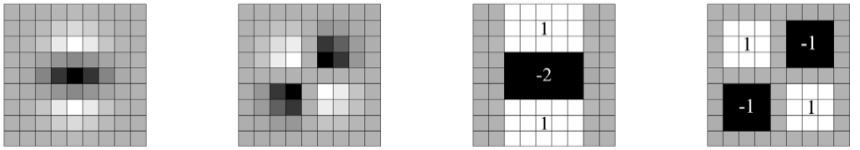
\includegraphics[scale=0.4]{bilder/surfBoxFilter.png}
    	\caption{Die Gaußfilter für die y und xy Richtung sowie deren Approximationen (Abbildung aus \cite{Bay:2008:SRF:1370312.1370556}).}
\label{fig:surfBox}
\end{figure} 


Um nun Keypoints in den verschiedenen Skalierungen zu finden, wird wie in SIFT geprüft, ob $det(\mathcal{H}(x, y, \sigma))$ an einem  Punkt in einer $3x3x3$ Nachbarschaft das Maximum ist.



\subsubsection{Merkmalsbeschreibung}

Der erste Schritt zur Erstellung des Deskriptors ist, dem Punkt eine Orientierung zuzuordnen. Sei $s$ im folgenden die Skalierung, in dem der Keypoint gefunden wurde.

Um dem Punkt eine Orientierung zuzuweisen, werden Haar Merkmale (siehe \ref{sec:haar}) verwendet. 
Es werden jeweils die Haar Merkmale in x und y Richtung bestimmt. Hierfür werden die Regionen in Abbildung \ref{fig:haar} mit einer Seitenlänge von $4s$ verwendet. Durch die Verwendung von Integralbildern sind diese Berechnungen sehr effizient.


Mit der gefunden Orientierung wird ein $20s$ großes Quadrat um den Punkt gelegt, welches um die Orientierung gedreht wird.
Dieses Quadrat wird in $4 \times 4$ Regionen unterteilt. In diesen Regionen wird ein 4-dimensionaler Merkmalsvektor bestimmt. Dieser Vektor besteht aus den Summen der horizontalen und vertikalen Haar Merkmale $dx$ und $dy$ in der Region(siehe Abbildung \ref{fig:surfFeature}). 
Die Größe der Regionen wird als $2s$ gewählt. Der Vektor ist definiert als: 

\begin{figure}[h]
    \centering
		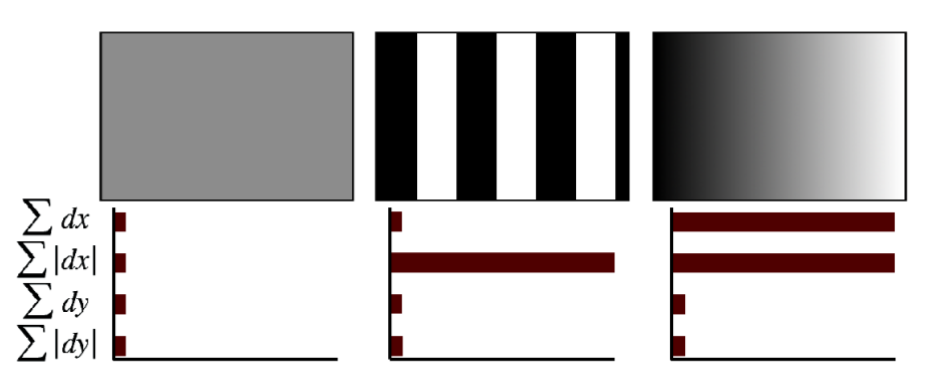
\includegraphics[scale=0.4]{bilder/surfFeature.png}
    	\caption{Die Größe der jeweiligen Merkmale für die gezeigten Bildausschnitte. Die einzelnen Komponenten des Vektors beschreiben die Strukturen der Intensität (Abbildung aus \cite{Bay:2008:SRF:1370312.1370556}).}
\label{fig:surfFeature}
\end{figure} 


\[
v = (\sum dx, \sum  |dx|, \sum dy, \sum |dy|)
\]

Aus den $4 \times 4$ Vektoren der einzelnen Regionen wird der Gesamtdeskriptor für das Merkmal gebildet.
Dadurch ensteht für jedes Merkmal ein 64-dimensionaler Vektor, der dieses Merkmal beschreibt.